\documentclass[11pt,onecolumn]{article}
\setlength{\columnsep}{0.5cm}

\usepackage[utf8]{inputenc}
\usepackage[T1]{fontenc}
\usepackage[spanish]{babel}
\usepackage{hyperref}
\usepackage{graphicx}
\usepackage{natbib}

\title{\vspace{-15mm}%
	\fontsize{24pt}{10pt}\selectfont
	\textbf{Estado del arte de la investigación sobre wikis}
	}	
\author{%
	\large
	\textsc{Emilio J. Rodríguez-Posada} \\
	\normalsize	Universidad de Cádiz \\
	\normalsize	\href{mailto:emiliojose.rodriguez@uca.es}{emiliojose.rodriguez@uca.es}
	\vspace{-5mm}
	}
\date{}


\begin{document}

\maketitle

\begin{abstract}

\end{abstract}

\section{Introducción}

En principio lo que voy a hacer es analizar el estado del arte de la investigación de wikis, contar WikiPapers, y un poco de mi trayectoria en estos temas, cuestiones abiertas, conclusiones y trabajo futuro.

Quizás para que fuera abordable el estado del arte, podría limitarme a clasificar los papers del último o dos últimos WikiSym. Y al último PAN/CLEF, WikiAI, MathWikis, Wikimania, WikiViz, etc. Comentar la existencia de todos estos eventos.

Reutilizar cosas que haya escrito ya en mis papers.

La intro la puedo adaptar del SLR que estoy haciendo de WikiPapers

\section{Motivación}

\section{Objetivos}

Hacer un estado del arte


\section{Definiciones, acrónimos y abreviaturas}

Mirar las que definí en mi PFC y meter otras más nuevas

\textbf{Administrador}:

\textbf{Anónimo}:


\textbf{API}:

\textbf{Artículo}:

\textbf{Blanqueo}:

\textbf{Bloqueo}:

\textbf{Bot}:

\textbf{Cambios recientes}:

\textbf{Cultura libre}:


\textbf{Dataset}:

\textbf{Diff}:


\textbf{Discusión}:

\textbf{Edición}:

\textbf{Espacio de nombres}:

\textbf{Etiqueta}:

\textbf{Expresión regular}:

\textbf{Fork}:


\textbf{GLAM}:

\textbf{Historial}:

\textbf{Interwiki}:

\textbf{Los cinco pilares}:


\textbf{Motor wiki}:

\textbf{Namespace}: véase \textbf{Espacio de nombres}.

\textbf{NPOV}: véase \textbf{Punto de vista neutral}.

\textbf{Política}:

\textbf{Preservación}:

\textbf{Proyectos hermanos}:

\textbf{Punto de vista neutral}:

\textbf{Regexp}: véase \textbf{Expresión regular}.

\textbf{Resumen de edición}:


\textbf{Reversión}:

\textbf{Robot}:


\textbf{Semántica}:

\textbf{Spam}:


\textbf{Usabilidad}:

\textbf{Vandalismo}:

\textbf{Web 2.0}:

\textbf{Wiki}:

\textbf{Wikifarm}:


\section{Estado del arte}

Áreas de investigación \href{http://wikipapers.referata.com/wiki/List_of_research_areas}{http://wikipapers.referata.com/wiki/List\_of\_research\_areas}

~\citep{okoli2009}
~\citep{martin2011}
~\citep{voss2005}
~\citep{okoli2009b}
~\citep{ayers2006}
~\citep{okoli2012}
~\citep{jullien2012}
~\citep{nielsen2011}


\subsection{Autoría y calidad}

WikiTrust, comparación Nature


\subsection{Cobertura y sesgos}


\subsection{Comunidad}


\subsection{Educación}


Wikis como herramientas educativas

Experiencias docentes

\subsection{Datasets}

\href{http://wikipapers.referata.com/wiki/List_of_datasets}{http://wikipapers.referata.com/wiki/List\_of\_datasets}


\subsection{GLAM}


\subsection{Herramientas}

\href{http://wikipapers.referata.com/wiki/List_of_tools}{http://wikipapers.referata.com/wiki/List\_of\_tools}

\subsection{Historiales}

\subsection{Infraestructura}

por ejemplo los wikis al estilo p2p para repartir la carga... había una tesis sobre eso en danés?


\subsection{Motivaciones e incentivos}


Encuestas...

\subsection{Motores wiki}


\subsection{Preservación}

urobe, revisar el paper de wikiteam

\subsection{Procesamiento de imágenes}

Poquísimo hay hecho me parece a mí...

\subsection{Procesamiento del Lenguaje Natural}


\subsection{Recomendación de tareas}

Images for bio

\subsection{Semántica}

SWEETpedia

\subsection{Usabilidad}

\subsection{Vandalismo y spam}

Bots y algoritmos, flaggedrevs, abusefilter, extensiones anti-spam

~\citep{avbot2011}
~\citep{avbot2010}
~\citep{avbot2009}

\subsection{Visualización}

WikiViz y todas las herramientas de visualización...


\subsection{Wikifarms}

~\citep{kittur2010}

\subsection{Wikis como redes sociales}


\section{Cuestiones abiertas}


\begin{figure}[htb]
\centering
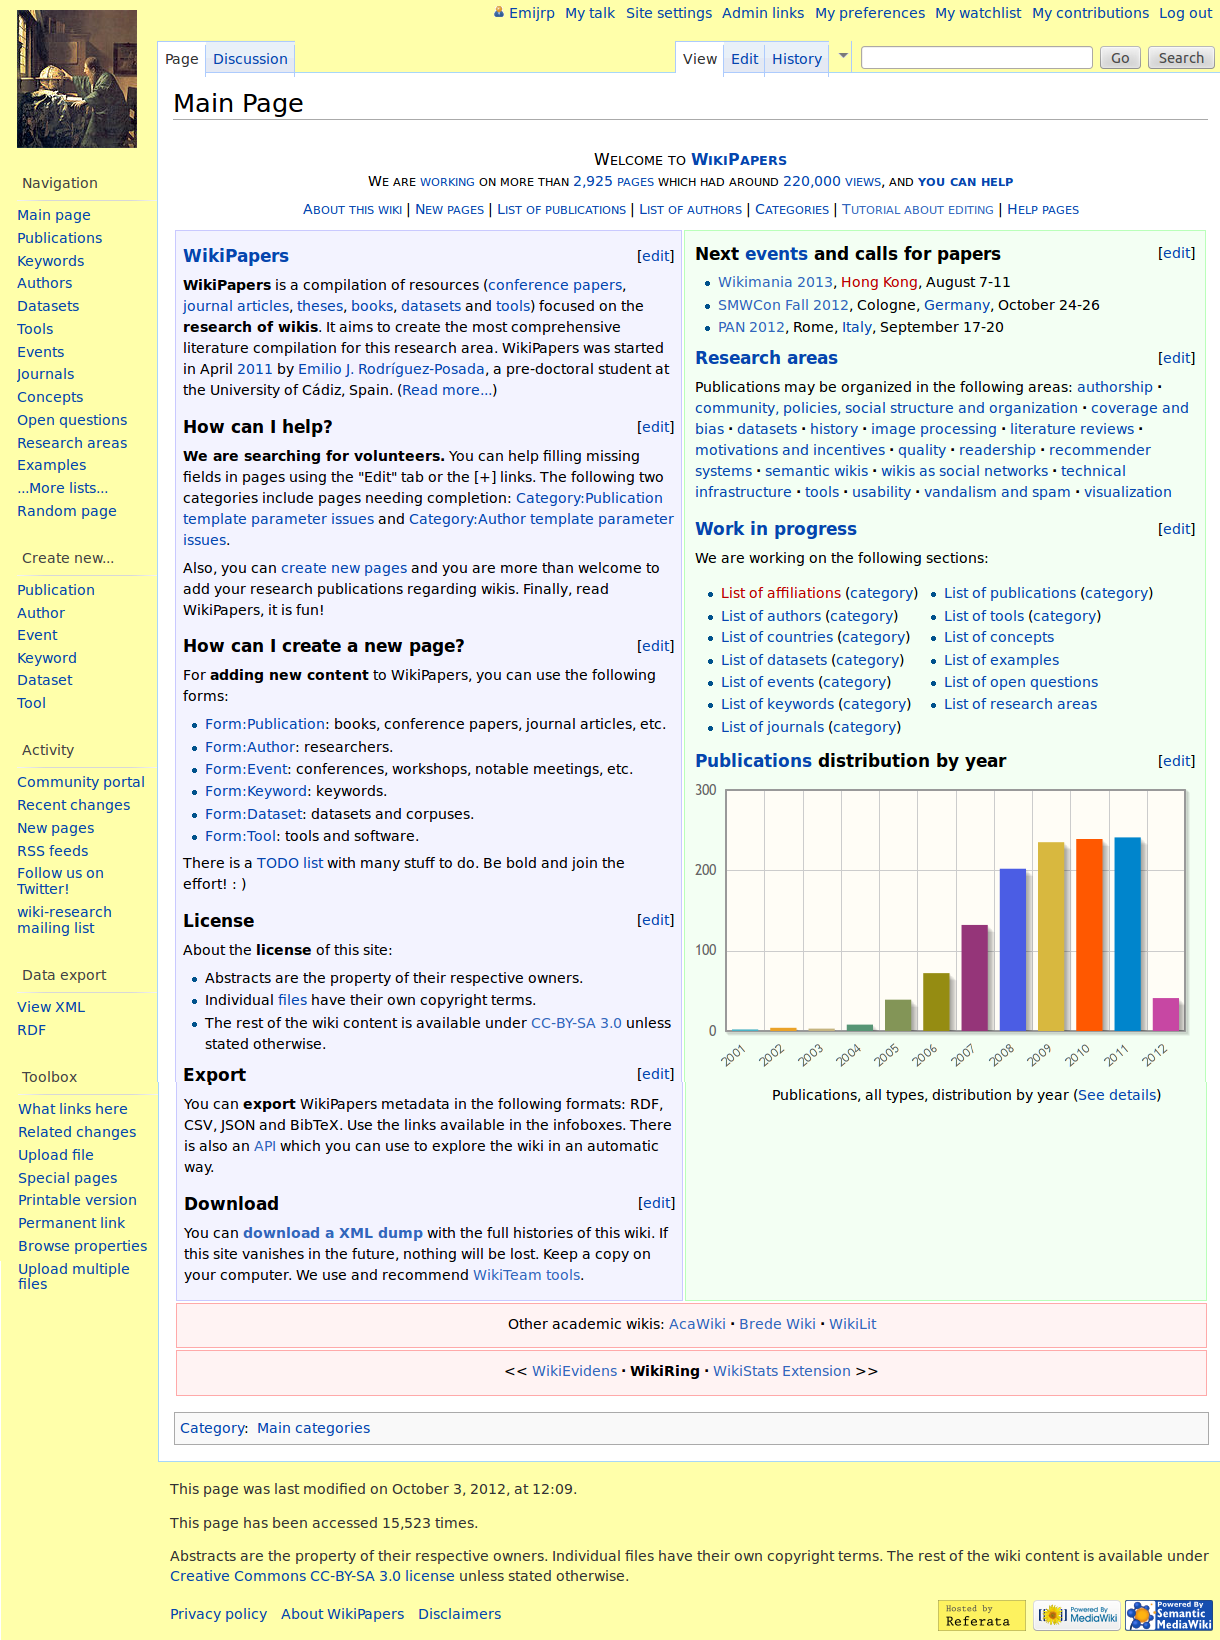
\includegraphics[width=0.8\textwidth]{wpfull.png}
\caption{Portada de WikiPapers}
\label{fig:wpfull}
\end{figure}


\section{Conclusiones y trabajo futuro}
porqué hacía falta WikiPapers
aglutina todas las ventajas de los anteriores sistemas
lo que se ha hecho, cifras,
lo que queda por hacer y como ayudar
el futuro y más allá...



\bibliographystyle{wink}        
\bibliography{proyecto-investigacion-2012}

\section*{Licencia}
Esta obra está bajo licencia \href{http://creativecommons.org/licenses/by-sa/3.0/}{Creative Commons Reconocimiento-CompartirIgual 3.0 Unported}.

\end{document}
